\chapter{The research: Development of a flight simulation model}

This chapter will focus on the work performed during the internship. It starts defining the main task and goals of the project and continues with a description of the methodology used. Then it focuses of the work done during the internship and finishes by presenting the end results.

\section{Problem statement}
Currently DAWN has began with the flight tests of their first research vehicle. As development is progressing the need for research into the \gls{cns} is growing. An important part in the development of these system are the flight models needed to tune controllers, aircraft design, systems software and hardware in the loop tests, etc. 

\subsection{Problem analysis and definition}
The development of these flight models is not easy, with the main problem being determining the aerodynamic properties of the aircraft. There are several options for determining the aerodynamic coefficients, each one with the own advantages and disadvantages.

\begin{itemize}
\item \textbf{Empirical models} \\ It is possible to get an estimate of the aerodynamic coefficients by using empirical models and tools. The advantage of these models is that they can quickly determine the aerodynamic coefficients for a wide range of flight conditions. However these tools are not accurate and can only be used for the early design stages.

\item \textbf{Computational models} \\ Another option is to calculate these coefficients based on numerical methods such as \gls{cfd} or potential flow. The main advantage is that they will give more accurate results than the empirical models and since no physical model is needed it's possible to change the design in order to optimize its flight characteristics. The disadvantages are that these methods can be computationally intensive and require special knowledge in order to perform them correctly.

\item \textbf{Wind tunnel} \\
Wind tunnel tests can give accurate estimates on the aerodynamic properties of the aircraft and since no full sized aircraft is needed it is still possible to perform changes to the aircraft. However wind tunnel availability and the limited number of flight conditions in which wind tunnel tests can be performed are the main problems.

\item \textbf{Real flight system identification} \\
The aerodynamic properties of the aircraft can also be determined using measurements taken during real flights. The main advantage is that if done correctly, these methods will give the most accurate estimate of the aerodynamic properties of the aircraft, which will give the information necessary to optimize the control systems. The main drawbacks are that a flight capable model is needed and the limited amount of flight data that can be collected.
\end{itemize}

Thus the main problem to be solved is: How can an accurate flight model be created with the resources currently available within DAWN.

\subsection{Goal and end product}
The end goal of the project is to research into the development of the tools necessary to create accurate flight simulation models. The end product will be a set of basic tools demonstrating the steps that need to be taken and a list of recommendations for the further development of these tools.

\section{Methodology}

\section{Work performed}
\subsection{Introduction and familiarization with the company and project}
The first step was to gain knowledge on the development that had already been done within DAWN, gather information on the current equipment and familiarize with the tools available.

\subsubsection{Current equipment}
The main flight computer being used on the current vehicle is the Pixhawk 2 running the Ardupilot autopilot software. The Pixhawk 2 is an open source flight computer designed by the Pixhawk open hardware community and thanks to its integrated sensors, redundant hardware and compact design it provides all the basic hardware needed to safely fly a small to medium sized drone. Ardupilot is a well developed open source autopilot software, it fully supports the Pixhawk 2 and provides the control, state estimation and navigation software needed to fly the current flight vehicle.

\subsubsection{Familiarization tasks}
Since the to be developed modeling tools would eventually have to be used with the Pixhawk and interface with Ardupilot two tasks where performed in order to familiarize with Ardupilot. The first tasks was the addition of new telemetry packages to the Ardupilot telemetry system. During this task basic knowledge was collected on the structure of the Ardupilot software and how to modify it. \\

The second task was setting up a \gls{sitl} test setup. This consisted of running the Ardupilot software on a development computer, in this case a laptop, and connect its sensor input, control outputs and telemtry outputs to a \gls{fdm} and a ground station software running on the same computer. The purpose of this setup is to provide an environment in which modifications to the Ardupilot software can be rapidly and safely tested without the need of the hardware. This allows the use of advanced software development tools that are not available for embedded systems, greatly simplifying the software development process without putting any of the equipment at risk. \\

Ardupilot's \gls{sitl} software package gives a wide range of options when it comes to the \gls{fdm} programs it can be connected to. Since further development of the simulation model synthesizing tools would depend on the \gls{fdm} chosen during this task a small trade-of was made to choose the appropriate tool for this stage of the project. The main points of interest for the \gls{fdm} where that it had to be easy to interface with from external software, easy to extend with new features, stable and accurate. \\

In the end JSBSim was chosen. JSBSim is an open source \gls{fdm} software library capable of modeling a wide range of aerospace vehicles. It's used by many open source flight simulation software packages most notably Flightgear and OpenEaagles and has been used on several university research projects around the world. The latest release contains all the features that will be necessary for the foreseeable future and its designed allows it to be easily extended or incorporated into other software tools. This is also the default \gls{fdm} for the Ardupilot SILT software and is thus the best supported one.

\subsection{Plan of approach}
After completing the familiarization tasks a plan of approach was made. As mentioned in the problem statement there are several options when it comes to determining the aerodynamic coefficients necessary to create the flight models. Wind tunnel tests and \gls{cfd} are not an option due to the limited time frame of the internship and the lack of expertise necessary to perform these. This leaves the empirical methods and system identification as the only options. \\

Empirical tools are able to quickly give an estimate of the aerodynamic coefficients, however these will be inaccurate and it is necessary to correct them if they will be used to design the control systems. Aerodynamic models based the system identification of real flight data are more accurate but since this requires the aircraft to be physically flown it limits the amount of flight data that can be collected. This can result in inaccuracies in the model or a model that is only valid for a limited set of flight conditions. \\

Thus the plan of approach is to combine both methods. The empirical tools will be used to create a large set of \textit{cheap} coefficients for a wide range of flight conditions and the \textit{expensive} coefficients will be determined with system identification of real flight data. This means that a tool to combine the two sets of coefficients will have to be developed.\\

Since the focus for now will be on the development of these tools. It is necessary to have a set of flight data for which the correct aerodynamic model is known. The easiest way to get such data is to calculate it using a simulation. Thus JSBSim will be used to generate this test data.\\

Digital Datcom is a freely available program capable if calculating the aerodynamic coefficients using empirical method, It is used to create the aerodynamic models used to develop the rest of the tools.\\

The two step method is chosen as the system identification method. This consists of 

\subsection{3rd party tools interface development}
To limit the amount of work necessary to complete these tasks, some third party software packages will be used. However since the to be developed tools will be written in Python it's necessary to make sure it is possible to interface with these tools from within a python script. The programs that will need interfaces are JSBSim and Digital Datcom.

\subsubsection{JSBSim}
JSBSim is an open-source \gls{fdm} software library written in C++ and by default provides no python bindings. So the first step was to look for existing python interfaces. The search revealed two possible options, "JSBSim Python" and "PyJSBSim". \\

Since the Sourceforge website was down at the time, the developer of "JSBSim Python" was directly contacted in order to get a copy of the source code and documentation. This revealed that the library had not been updated since 2007 and that it would probably require modifications in order to make it run with the current versions of JSBSim and Python. \\

Development for PyJSBSim is not active either, but the JSBSim development team uses it as part of their unit tests. Thus the copy of PyJSBSim in the JSBSim code repository is guaranteed to work with the current version of JSBSim. However PyJSBSim only implements a small subset of the JSBSim API and it doesn't give the option to create new aircraft models from within python since these consists of \gls{xml} files that need to be manually created before running the simulation. \\

Thus the next step was to extend PyJSBSim to include the extra features that would be needed and create a set of functions capable of creating the JSBSim aircraft model \gls{xml} files. PyJSBSim is written in Cython, a static compiler for Python and the extended Cython programming language. Code written in Cython can seamlessly interact with C/C++ and Python code, making it the perfect tool to write interfaces between Python and C++ code. \\

The first modifications where to make PyJSBSim run properly in Python 3. The code was already running, but because of changes in the language some extra type conversions where necessary in order to make the Python side of the interface easier to work with. One important feature that had to be added was the ability to give JSBSim tables with predetermined the control inputs. The rest of the changes made to PyJSBSim consisted of exposing a few more C++ functions and classes to Python and annotating the Cython code with type information.\\

As mentioned before, a tool had to be developed in order to to create the JSBSim aircraft models from within Python code. Since the input files contain \gls{xml} code, Jinja2, a templating language for Python, was chosen to write \gls{xml} template files that could then be filled in from the python code. \\

However before development of this tool could start, the aerodynamic model had to be defined. The reason for this is because JSBSim does not have an aerodynamic model. Instead the equations to calculate the aerodynamic forces need to be given in the input \gls{xml} files. To keep it simple, the linear model described in the TU Delft Flight dynamics course was used as the basis \cite{fdreader}. \\

The aerodynamic forces and moments are calculated using equations \autoref{eq:f_a} and \autoref{eq:m_a}. The aerodynamic coefficients in the body reference frame are defined in \autoref{eq:body_coefs} and the dimensionless rates used in \autoref{eq:body_coefs} are defined in \autoref{eq:dim_less_rates}.

\begin{equation}
\label{eq:f_a}
{F_A} = \frac{1}{2}\rho V_{tas}^2S\left[ {\begin{array}{*{20}{c}}
{{C_X}}\\
{{C_Y}}\\
{{C_Z}}
\end{array}} \right]\\
\end{equation}

\begin{equation}
\label{eq:m_a}
{M_A} = \frac{1}{2}\rho {V^2}S\left[ {\begin{array}{*{20}{c}}
{{C_l} \cdot b}\\
{{C_m} \cdot \bar c}\\
{{C_n} \cdot b}
\end{array}} \right]
\end{equation}

\begin{equation}
\label{eq:body_coefs}
\arraycolsep=1.4pt\def\arraystretch{2.2}
\begin{array}{l}
{C_X} = C_{{X_0}} + ({C_{{X_u}}} - 2\;{C_{{X_0}}})\;\hat u + {C_{{X_\alpha }}}\alpha  + {C_{{X_{{\alpha ^2}}}}}{\alpha ^2} + C_{{X_{\dot{\alpha}}}}\hat{\dot{\alpha}}  + {C_{{X_q}}}\hat q + {C_{{X_{{\delta _e}}}}}{\delta _e}\\
{C_Y} = {C_{{Y_\beta }}}\beta  + {C_{{Y_p}}}\hat p + {C_{{Y_r}}}\hat r + {C_{{Y_{{\delta _a}}}}}{\delta _a} + {C_{{Y_{{\delta _r}}}}}{\delta _r}\\
{C_Z} = ({C_{{Z_u}}} - 2\;{C_{{Z_o}}})\;\hat u + {C_{{Z_\alpha }}}\alpha  + {C_{{Z_{\dot{\alpha}}}}\hat{\dot{\alpha}} + {C_{{Z_q}}}\hat q + C_{{Z_{{\delta _e}}}}}{\delta _e}\\
{C_l} = {C_{{l_\beta }}}\beta  + {C_{{l_p}}}\hat p + {C_{{l_r}}}\hat r + {C_{{l_{{\delta _a}}}}}{\delta _a} + {C_{{l_{{\delta _r}}}}}{\delta _r}\\
{C_m} = {C_{{m_u}}}\hat u + {C_{{m_\alpha }}}\alpha  + C_{{m_{\dot{\alpha}}}}\hat{\dot{\alpha}}  + {C_{{m_q}}}\hat q + {C_{{m_{{\delta _e}}}}}{\delta _e}\\
{C_n} = {C_{{n_\beta }}}\beta  + {C_{{n_p}}}\hat p + {C_{{n_r}}}\hat r + {C_{{n_{{\delta _a}}}}}{\delta _a} + {C_{{n_{{\delta _r}}}}}{\delta _r}
\end{array}
\end{equation}

\begin{equation}
\label{eq:dim_less_rates}
\arraycolsep=1.4pt\def\arraystretch{2.2}
\begin{array}{l}
\hat u = \frac{{u - V}}{V}\\
\hat{\dot{\alpha}} = \frac{\dot{\alpha}\bar{c}}{V}\\
\hat p = \frac{{pb}}{{2V}}\\
\hat q = \frac{{q\bar c}}{V}\\
\hat r = \frac{{pb}}{{2V}}
\end{array}
\end{equation}

Since the aircraft is assumed to be trimmed at the beginning of the simulation, It is assumed that the thrust equals the aerodynamic drag. Thus the thrust and the aerodynamic force coefficient term $C_{x_0}$ cancel each other out. The $C_{x_0}$ term can then be removed from the equation and it is not necessary to give JSBSim the engine thrust. Thus the new equation for the $C_X$ coefficient can be written as in \autoref{eq:c_x}

\begin{equation}
\label{eq:c_x}
{C_X} = ({C_{{X_u}}} - 2\;{C_{{X_0}}})\;\hat u + {C_{{X_\alpha }}}\alpha  + {C_{{X_{{\alpha ^2}}}}}{\alpha ^2} + C_{{X_{\dot{\alpha}}}}\hat{\dot{\alpha}}  + {C_{{X_q}}}\hat q + {C_{{X_{{\delta _e}}}}}{\delta _e}
\end{equation}\\

In order to check whether the aerodynamic model is correct it is necessary to compare the simulation results with a different simulation. To do this the \gls{lti} model from the flight dynamics reader\cite{fdreader} has been chosen. This model is defined in Equations \ref{eq:lti_sym} and \ref{eq:lti_asym}. The equations for the elements these matrices are given in \autoref{fig:completetable}. The coefficients used in the test are those for the Cessna Ce500 'Citation' during cruise and are given in \autoref{fig:coeftable}\\


\begin{equation}
\label{eq:lti_sym}
\left[ {\begin{array}{*{20}{c}}
    {\dot u} \\ 
    {\dot \alpha } \\ 
    {\dot \theta } \\ 
    {\dot q} 
\end{array}} \right] = \underbrace {\left[ {\begin{array}{*{20}{c}}
    {{x_u}}&{{x_\alpha }V}&{{x_\theta }V}&0 \\ 
    {{z_u}\tfrac{1}{V}}&{{z_\alpha }}&{{z_\theta }}&{{z_q}\tfrac{{\bar c}}{V}} \\ 
    0&0&0&1 \\ 
    {{m_u}\tfrac{1}{{\bar c}}}&{{m_\alpha }\tfrac{V}{{\bar c}}}&{{m_\theta }\tfrac{V}{{\bar c}}}&{{m_q}} 
\end{array}} \right]}_{{A_{symmetric}}}\left[ {\begin{array}{*{20}{c}}
    u \\ 
    \alpha  \\ 
    \theta  \\ 
    q 
\end{array}} \right] + \underbrace {\left[ {\begin{array}{*{20}{c}}
    {{x_{{\delta _e}}}V} \\ 
    {{z_{{\delta _e}}}} \\ 
    0 \\ 
    {{m_{{\delta _e}}}\tfrac{V}{{\bar c}}} 
\end{array}} \right]}_{{B_{symmetric}}}{\delta _e}
\end{equation}




\begin{equation}
\label{eq:lti_asym}
\left[ {\begin{array}{*{20}{c}}
    {\dot \beta } \\ 
    {\dot \varphi } \\ 
    {\dot p} \\ 
    {\dot r} 
\end{array}} \right] = \underbrace {\left[ {\begin{array}{*{20}{c}}
    {{y_\beta }}&{{y_\varphi }}&{{y_p}\tfrac{b}{{2V}}}&{{y_r}\tfrac{b}{{2V}}} \\ 
    0&0&1&0 \\ 
    {{l_\beta }\tfrac{{2V}}{b}}&0&{{l_p}}&{{l_r}} \\ 
    {{n_\beta }\tfrac{{2V}}{b}}&0&{{n_p}}&{{n_r}} 
\end{array}} \right]}_{{A_{asymmetric}}}\left[ {\begin{array}{*{20}{c}}
    \beta  \\ 
    \varphi  \\ 
    p \\ 
    r 
\end{array}} \right] + \underbrace {\left[ {\begin{array}{*{20}{c}}
    0&{{y_{{\delta _r}}}} \\ 
    0&0 \\ 
    {{l_{{\delta _a}}}\tfrac{{2V}}{b}}&{{l_{{\delta _r}}}\tfrac{{2V}}{b}} \\ 
    {{n_{{\delta _a}}}\tfrac{{2V}}{b}}&{{n_{{\delta _r}}}\tfrac{{2V}}{b}} 
\end{array}} \right]}_{{B_{asymmetric}}}\left[ {\begin{array}{*{20}{c}}
    {{\delta _a}} \\ 
    {{\delta _r}} 
\end{array}} \right]
\end{equation}

\begin{figure}
\centering
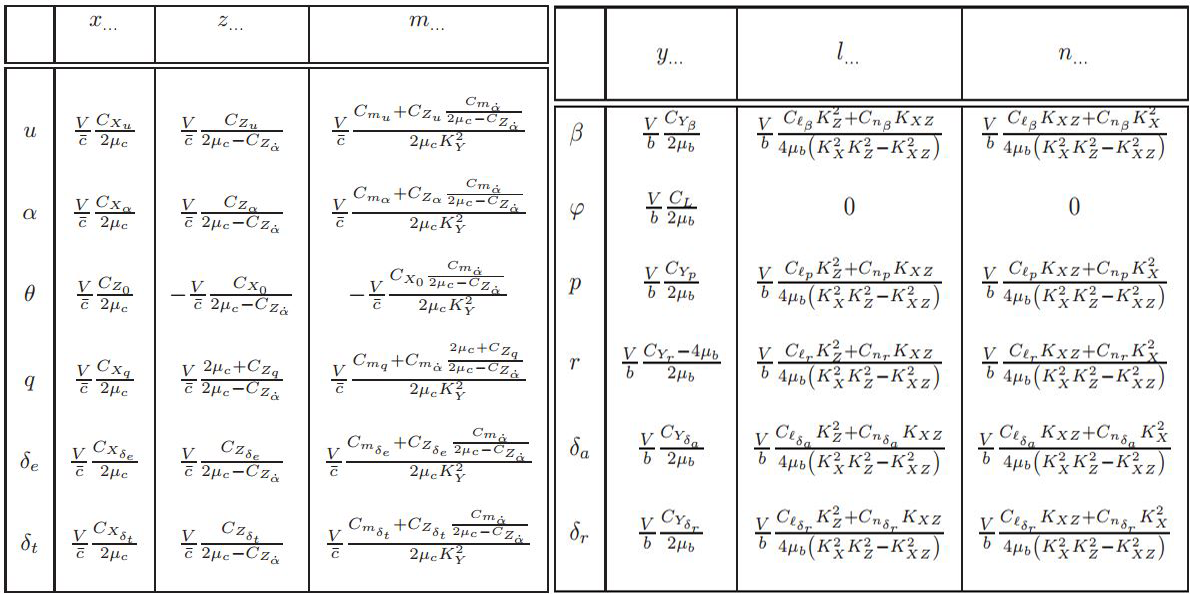
\includegraphics[width=14cm]{figures/tablecomplete.png}
\caption{Coefficient table for the symmetric (left) and the asymmetric (right) modes.}
\label{fig:completetable}
\end{figure}

\begin{figure}
\centering
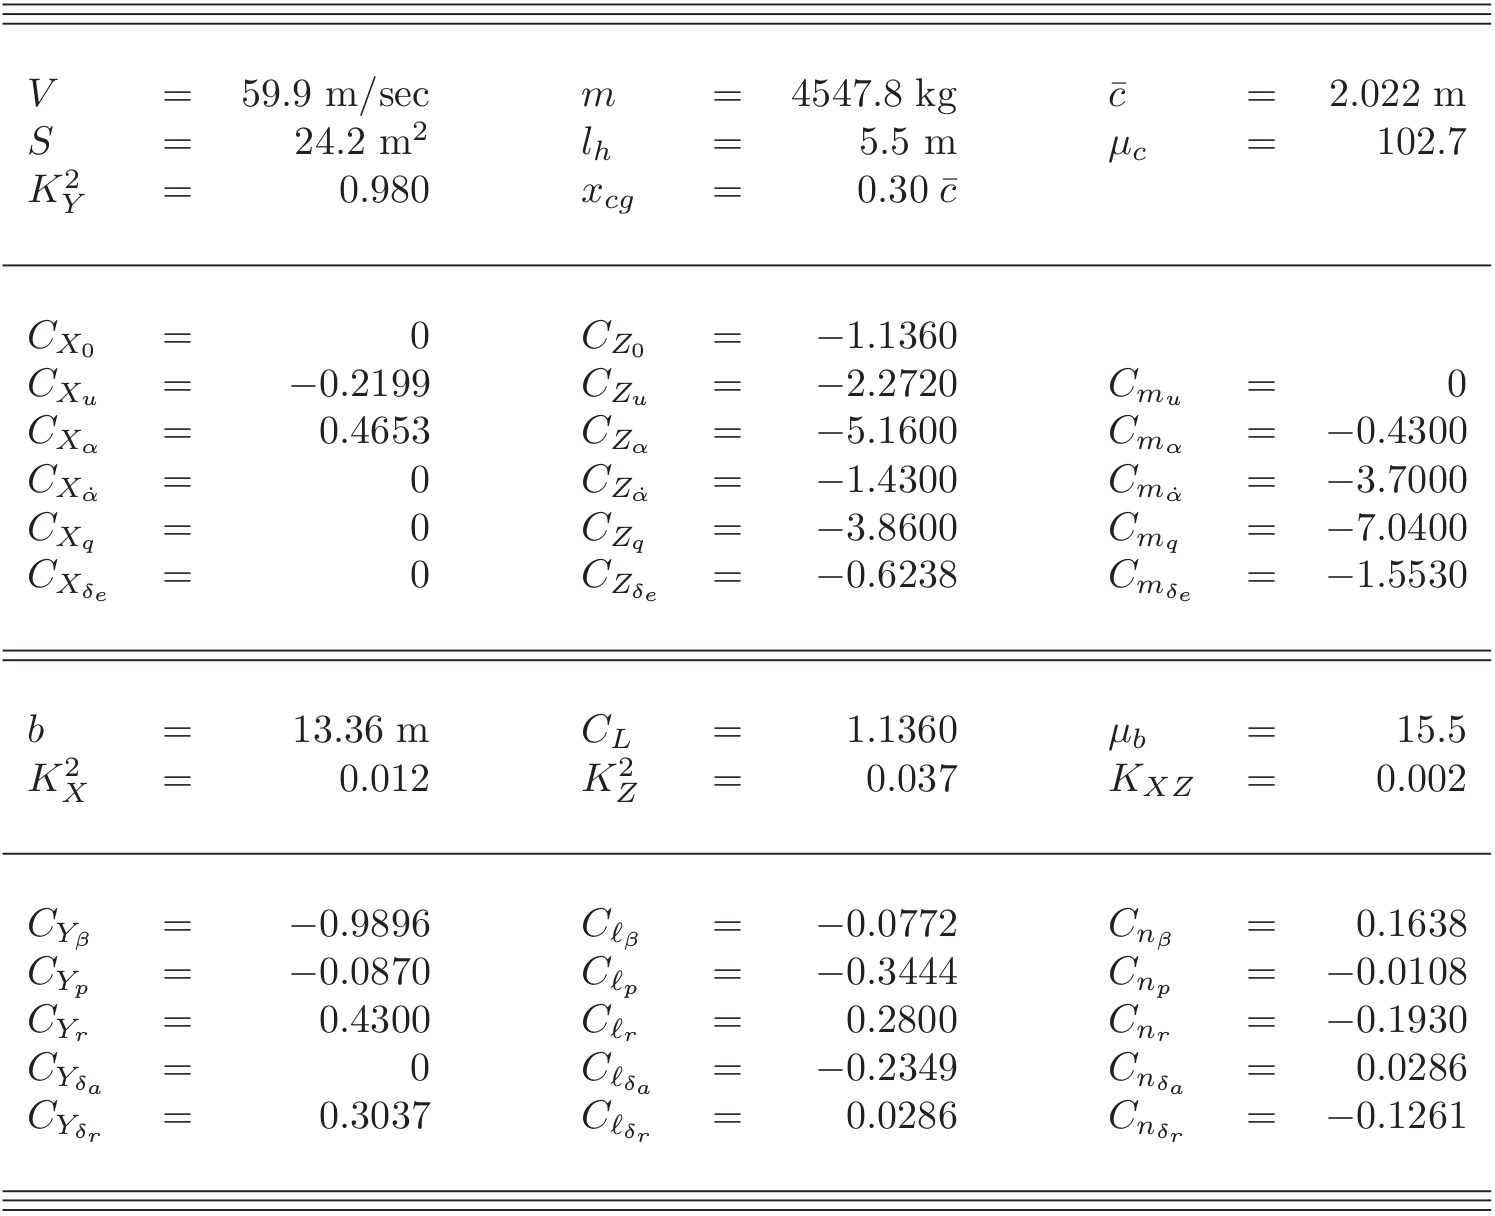
\includegraphics[width=14cm]{figures/tablecoefs.png}
\caption{Symmetric and asymmetric stability and control derivatives for the Cessna Ce500 ‘Citation’, Cruise}
\label{fig:coeftable}
\end{figure}


A JSBSim input file was manually created with the aerodynamic model given above with the values for the Citation where filled in. The results are shown in Figures~\ref{fig:lti_elevator},~\ref{fig:lti_aileron}~and~\ref{fig:lti_rudder}. As it can be seen the JSBSim and the \gls{lti} system give roguhly the same results, specially in the first few simulation seconds. Thus the JSBSim model is deemed good enough to be used to generate test flight data.


\begin{figure}
\centering
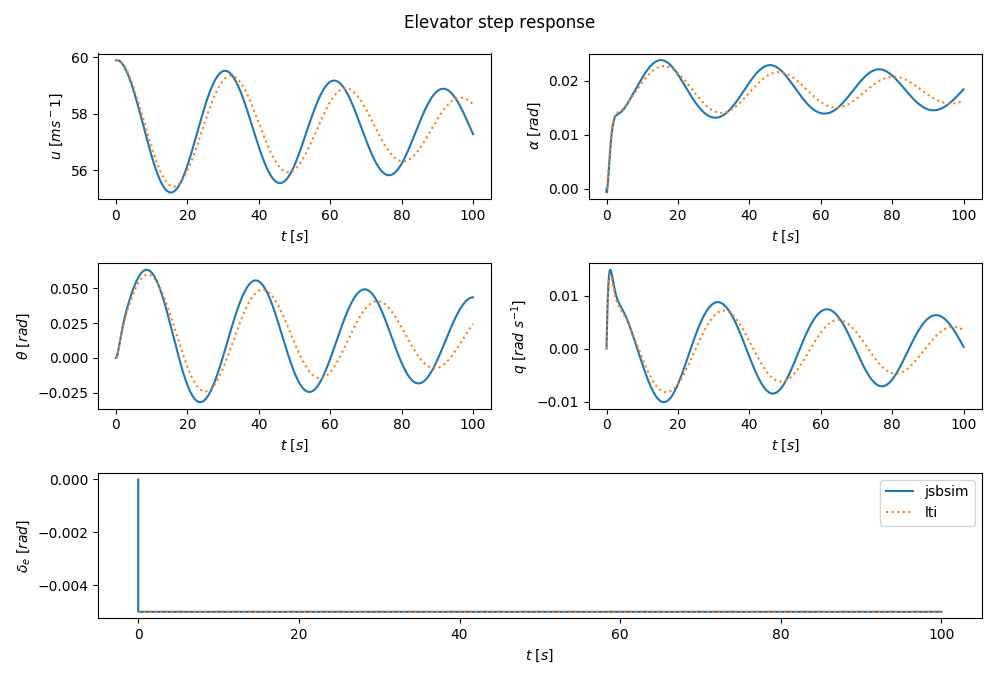
\includegraphics[width=14cm]{figures/lti_elevator}
\caption{Response curves for a step elevator deflection ($\Delta\delta_e=-0.005\ [Rad]$ calculated by JSBSim and the \gls{lti} model.)}
\label{fig:lti_elevator}
\end{figure}

\begin{figure}
\centering
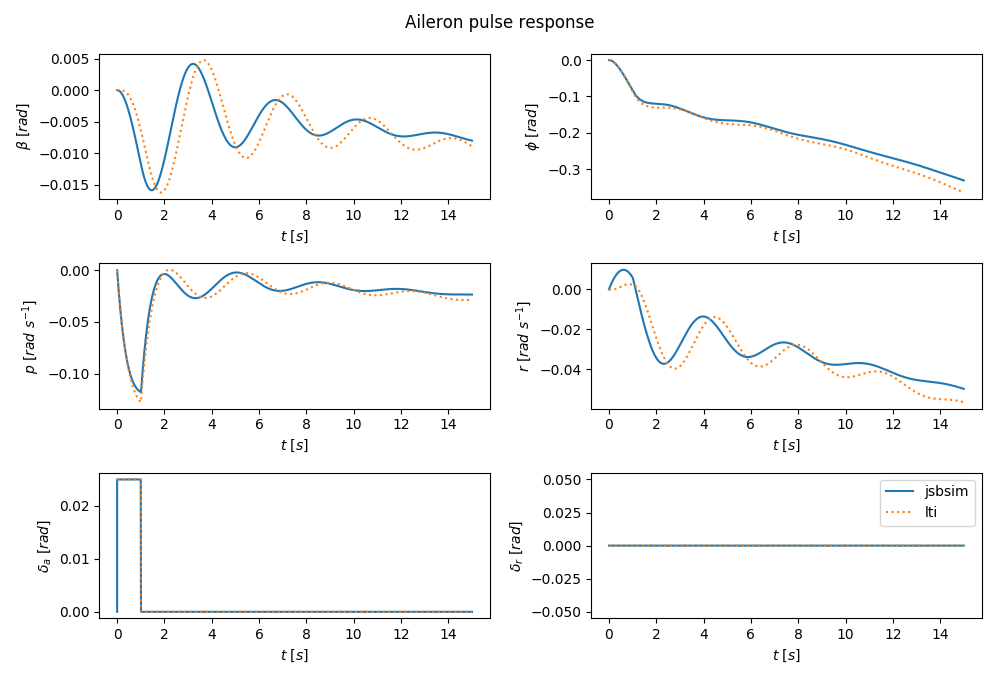
\includegraphics[width=14cm]{figures/lti_aileron}
\caption{Response curves for a pulse shaped aileron deflection ($\Delta\delta_a=0.025\ [Rad]$ calculated by JSBSim and the \gls{lti} model.)}
\label{fig:lti_aileron}
\end{figure}

\begin{figure}
\centering
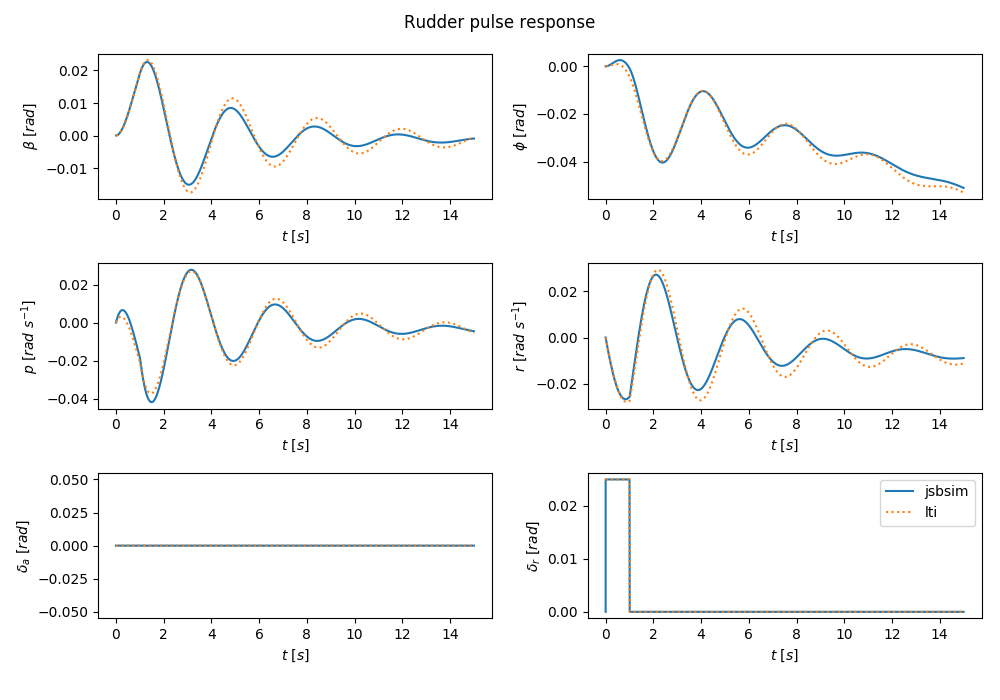
\includegraphics[width=14cm]{figures/lti_rudder}
\caption{Response curves for a pulse shaped rudder deflection ($\Delta\delta_r=0.025\ [Rad]$ calculated by JSBSim and the \gls{lti} model.)}
\label{fig:lti_rudder}
\end{figure}


\subsubsection{Digital Datcom}
Digital Datcom is a program capable of calculating the aerodynamic coefficients using empirical methods contained in the \gls{usaf} Stability and Control Datcom (Data Compendium). The source code for Digital Datcom is available online, however Digital Datcom is written in Fortran. Thus it has been decided to create the Python wrapper around a pre-compiled executable. Datcom+ has thus been chosen. Datcom+ is a modified variant of Digital Datcom which has been extended with extra tools and output formats and is available as a pre-compiled binary file.\\

The Datcom+ wrapper is simple. It consists of a template file with the geometry of the Cessna Ce550 'Citation~II'. The flight conditions and control inputs are left blank since these are filled in by the Python wrapper. This however means that the current wrapper can only generate coefficients for the Citation II. It will thus be necessary to extend this wrapper in the future, but for now it is enough to test and demonstrate the tools being developed.\\

One drawback of Digital Datcom is that not all coefficients can be calculated using it. $C_{X_{\alpha^2}}$ is calculated by fitting a second order polynomial on the value of $C_X$ at different angles of attack. The value of $C_{X_{\alpha^2}}$ will then be the value of the highest order term of the polynomial as it's shown in \autoref{eq:c_x_alpha2}\\

\begin{equation}
\label{eq:c_x_alpha2}
{C_X}(\alpha ) = {C_{X_{\alpha ^2}}}{\alpha ^2} + {C_{{X_\alpha }}}\alpha  + {C_{{X_0}}}
\end{equation}
 
The rest of the unknown coefficients are either left at zero or a value is chosen such that the resulting model is stable. Keep in mind the goal is to generate aerodynamic models that can be used to test the system identification and coefficient mixing tools and are not required to accurately represent a real aircraft. \\

Since the goal is to simulate an aircraft, more information is needed besides the aerodynamic coefficients. These are the masses, reference area, lengths, etc. most of this information has been collected from 'Jane's All The World's Aircraft: Development \& Production' \cite{janes}. However it was not possible to find a reference containing the \gls{mmoi} for the Citation II. It was thus decided to estimate the \gls{mmoi} using the Class I method described in 'Airplane Design Part V: Component Weight Estimation' by J.~Roskam\cite{roskam_5}. These are Equations~\ref{eq:ros_ixx},~\ref{eq:ros_iyy}~and~\ref{eq:ros_izz}.


\begin{equation}
    \label{eq:ros_ixx}
    {I_{XX}} = {b^2}\bar R_X^2\frac{W}{{4g}}
\end{equation}
\begin{equation}
    \label{eq:ros_iyy}
    {I_{YY}} = {L^2}\bar R_Y^2\frac{W}{{4g}}
\end{equation}
\begin{equation}
    \label{eq:ros_izz}
    {I_{ZZ}} = {e^2}\bar R_Y^2\frac{W}{{4g}}
\end{equation}

Where b and L are the wingspan and overall length of the aircraft and e is given by \autoref{eq:ros_e}.

\begin{equation}
    \label{eq:ros_e}
    e = \frac{{b + L}}{2}
\end{equation}

The non-dimensional radius of gyration $\bar{R}_X$, $\bar{R}_Y$ and $\bar{R}_Z$ tends to be the same for aircraft with the same mission orientation. This assumption is however not necessary in the case of the Citation II, since a table with the non-dimensional radius of gyration is available for this aircraft.\cite{roskam_5}\\

Unfortunately there is no Class I method to determine $I_{XZ}$, thus a Class II analysis is necessary to determine it's value. Since this type of analysis would take to much time and insufficient information on the Citation~II is known, it has been decided to assume a fixed value of $2483.2\ [Kg\ m^2]$. This was calculated by using the same value for $K_{XZ}$ as of the Citation.
























































